\chapter{绪论}
\label{chap:myIntro}

\section{研究背景及意义}
\label{sec:background}
增强现实(Augmented Reality,AR)是一种利用计算机生成视觉、听觉等感官信息,然后与真实世界中的物体进行混合,最终呈现在用户面前的技术。\cite{ARconception}

目前增强现实在很多领域都有使用,例如在游戏领域,增强现实技术可以改变传统游戏的交互方式,为玩家提供更加新奇的游戏体验。
    
\begin{figure}[!htp]
  \centering
  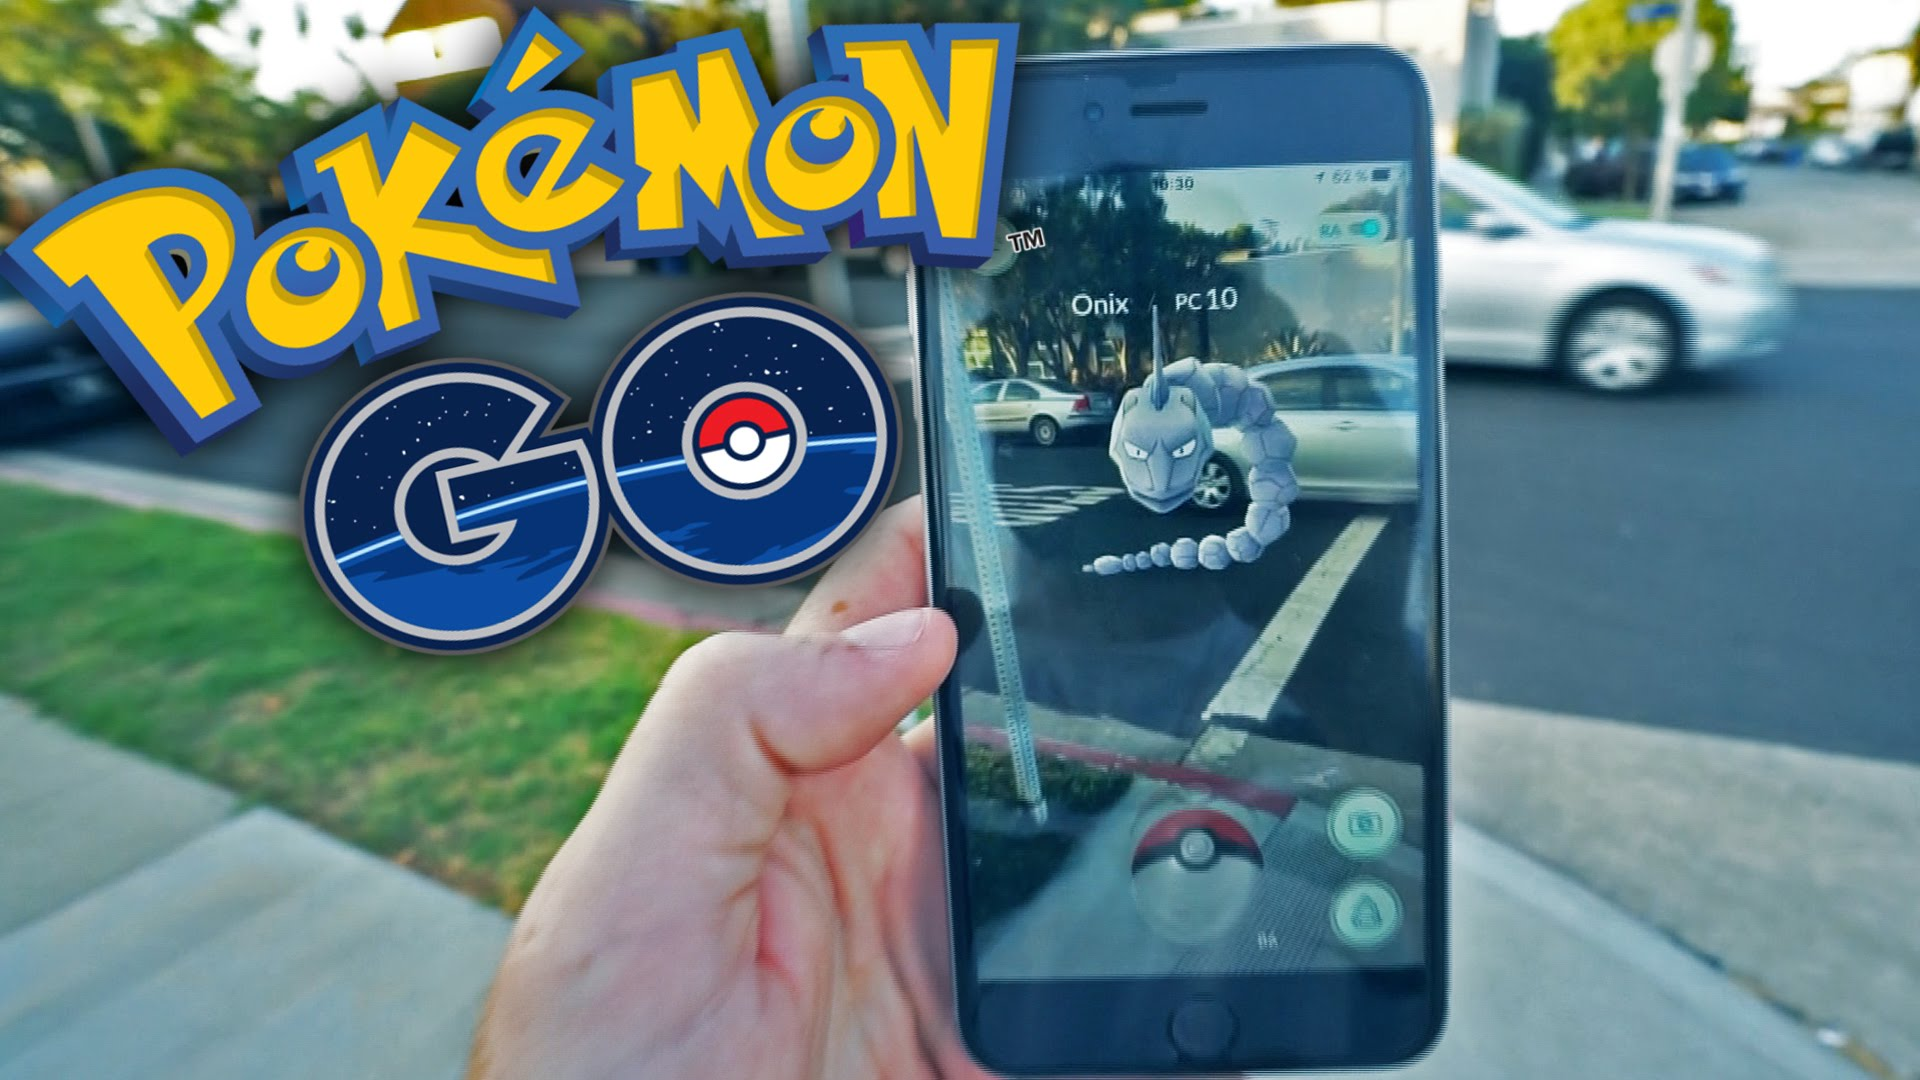
\includegraphics[width=12cm]{pokemongogaming.jpg}
  \bicaption[AR游戏 Pokemon Go海报]
    {AR游戏 Pokemon Go海报}
    {The wallpaper of AR game Pokemon Go}
 \label{fig:longcaptionbad}
\end{figure}

在实际应用中,增强现实也被广泛应用于提供辅助信息。例如在汽车领域,增强现实技术能够在驾驶过程中为驾驶员提供导航、路况提醒等信息。\cite{ARdriving}在医学领域,可以通过AR技术将超声波图像显示在患者身体上为医生提供更多信息。\cite{billinghurst2002augmented}

增强现实技术也逐渐被应用在教育领域,为教师和学生提供更加丰富的教学内容。目前的实验教学存在诸多问题,例如,实验条件(器材、空间、教师、开放时间)有限,学生动手操作和试错的机会少,实验指导不能随着实验进行实时提示与更新等问题。而增强现实技术因为可以可视化抽象概念,模拟复杂的现象,提供模拟实验练习等优势,因此被广泛应用。\cite{wu2013current}但是,教育领域与上述其他领域不同的是,用户(教师)也是软件开发的一部分,需要具有自主编辑实验的自由。但是教师由于通常不具备软件开发能力,因此需要应用提供一套用户友好的编著系统。

与此同时,处于为用户提供更丰富的交互体验,例如为用户提供触觉,或将显示信息与可交互的物体进行更好融合的目的,增强现实应用往往需要的实现对于物体的识别和追踪。

本文旨在开发一套增强现实辅助教学应用,在后端通过物体追踪,为用户提供具有真实触感的交互体验,并且在交互过程中显示物体的辅助信息。在前端开发一套用户友好的编著系统,为非计算机专业人士编辑用于教学的增强现实应用。

这套系统的意义在于,教育者可以在花费较少的学习成本的前提下,自主创建、编辑实验,并且结合现实器材,为学生提供多样的模拟实验。在教学过程中,教育者减少了教学、演示、实验指导的负担,学生实验可以不再受器材、人员等因素的限制,在保证安全的同时有大量误操作、试错的机会,可以更好的学习实验。而与增强现实技术相结合,该系统可以使学生拥有多种感官的体验,模拟实验更加逼真。



\section{国内外研究现状}
\subsection{物体追踪}
在增强现实应用中,出于融合需要,往往需要对真实物体进行物体姿态检测和追踪。目前很多学者在这方面做出了研究。基于模型的物体追踪可以分为两类,基于RGB-深度图像和仅基于RGB图像。

对于基于RGB图像进行物体姿态检测的研究,目前使用较多的、可以达到实时效果的是基于模式匹配(template matching)的方法。例如Hinterstoisser等人提出的LINE方法\cite{hinterstoisser2011gradient},在传统的使用图像和梯度(gradients)检测物体的模式匹配方法的基础上,通过依靠局部优势梯度方向(local dominant gradients orientation)建立模式不变量,并且考虑梯度方向在图片中的相邻区域。通过上述两者结合来数学表示输入图像,之后进行模式识别,可以获得更加稳定和高效的追踪效果。此外,近年来也有一些基于学习的方法进行物体姿态检测的研究被提出。例如,Brachmann等人提出的,基于随机森林(random forest)扩展的方法。\cite{brachmann2016uncertainty}但是由于选择的特征会在很大程度上影响决定姿态的投票数量,基于随机森林的方法在性能上往往并不能达到实时的要求。

而对于基于RGB图像进行物体追踪的方法来说,最早能够够达到实时要求的是算法是Prisacariu和Reid提出的PWP3D算法\cite{prisacariu2012pwp3d}。该算法构建了一个概率框架,将前景部分使用符号距离函数进行描绘,并且定义了该区域的能量。而后景部分则基于像素级别的后验隶属概率进行描绘。之后这个方法被Hexer等人发展为利用局部颜色直方图进行前后景分隔,提升了效率。\cite{hexner20162d}

但是仅使用RGB图像进行物体追踪的技术相比于添加深度图像进行辅助仍然有所欠缺。例如LINE方法\cite{hinterstoisser2011gradient}在有深度信息的时候,可以通过获得物体的表面法向量来进一步提升鲁棒性。而Brachmann的方法\cite{brachmann2016uncertainty}也通过边缘化物体坐标分布的深度值,从而弥补深度值的缺失,实现追踪。相比之下,结合深度值的方法则更加成熟与稳定。

在物体检测方面,传统的方式可以分为基于模式和基于特征两种。上述的基于模式匹配的LINE方法\cite{hinterstoisser2011gradient}在加入深度信息辅助,以及其他的类似方法\cite{kehl2016hashmod, rios2013discriminatively}, 都可以实现基于RGB-D图像的物体检测。但是这些方法在检测多个物体的时候计算率都是呈线性增长的,可扩展性较差。而基于特征的方法,最早是通过RGB图像获得特征\cite{lowe2004distinctive},然后反向投影到三维坐标中的\cite{lowe2001local}。在三维描述符引入后,则可以直接通过三维点云计算特征点\cite{mian2010repeatability}。从而获得比较好的延展性,但这些方法的性能往往并不能达到实时的要求。在机器学习发展之后,出现了基于随机森林投票确定物体姿态的方法。\cite{brachmann2016uncertainty, tejani2014latent}前者是使用能量函数进行姿态估测,而后者则是使用投票机制。在这之后,也出现了基于卷积神经网络(convolutional neutral network, CNN)进行姿态识别的研究\cite{kehl2016deep}.该方法使用了局部取样的RGB-D图像补丁(patch)进行神经网络训练,然后在使用的时候通过补丁描述符进行匹配推测物体姿态。

而在物体追踪方面,目前的方法大多数都是基于已知待追踪模型的数据的。他们通过构造图像的函数,描绘观测图像和目标图像之间的差别,将构造函数最小化从而确定物体姿态。一种处理图像数据的方式是迭代最近点算法(iterative closest point, ICP)。他的目的是通过找到待配准点云数据(追踪时获取的数据)与参考点云数据(物体模型数据)之间的旋转和平移关系,进行最优匹配。Held实现的物体追踪算法就使用了这个方法。\cite{held20123d}但是在多物体追踪时候往往需要进行预分隔,必须使用一个不同的模型,在应对多物体的时候效果并不好。
另一种替代ICP的方法是符号距离函数(Signed Distance Function, SDF)。他描绘了点云和物体模型的关系。本文实现的物体追踪系统使用了Ren等人基于SDF实现的物体追踪算法。\cite{ren2017real}他们通过描绘物体的SDF函数,构造代价函数,求解物体姿态。具体算法将会在相关技术中详细分析。

\subsection{虚拟场景中的编著系统}
目前针对用户自主编辑虚拟场景的需求,有许多应用面市。例如基于互联网交互游戏Second life的编程语言Linden Scripting Language(LSL),是用户·可以·通过简单的编程,就可以实现在虚拟场景中自定义与其他物体的交互。\cite{LSLTutorial}在此基础上,也有很多应用,方便用户进行简单的编程之后生成代码导入second life,如Particle,Dialog Menu, MiceOnABeam Visual Scripting Tool等等。\cite{zhong2014domain}这些工具虽然便利了用户使用虚拟场景,但是仍然需要用户具备一定的编程能力,距离实际教师教学仍有一定差距。

在这之后,有许多虚拟场景中的模拟程序被开发,例如Ying Zhong等人开发的化学模拟实验引擎。\cite{zhong2014domain}用户可以创建、编辑、操纵化学实验用具,通过·TCP/IP与服务器和数据库联通。工具具有比较好的易用性,但是体现化学专业知识、进行操作提示的部分比较少,交互方式也比较局限,并且只局限在PC端。此外,牛津大学也开发了一款用于教学的化学实验模拟引擎,虽然引擎本身对于化学实验及其原理、实验操作都有比较详细的讲述,但是由于演示使用过视频片段整合形成的,交互方式非常局限。\cite{OxfordChe}在这之后,Ali等人开发了一套化学实验模拟引擎系统,\cite{ali2014effect}将上述两者整合起来,既支持比较多的交互方式,还支持化学知识的教学。除此以外,虚拟场景编辑也应用在了物理等其他自然科学领域。\cite{daineko2017using}

虽然编著系统已经有广泛的应用,但是从上述软件可以看出,交互方式仍然局限在电脑屏幕,而且对于实验环境的编辑也比较缺乏。

\section{本文主要工作}
本文开发了一套增强现实应用,前端基于Unity引擎开发,为教育者提供了一个可以创建实验、调节实验环境的编著系统,后端通过Kinect获取RGB-D图像,基于上述的Ren提供的算法\cite{ren2017real}实现对特定模型的追踪,并结合Vuforia工具辅助,在Unity场景中渲染,从而达到虚实融合,具有真实触感的增强现实应用。


\section{本文结构}
本文一共分为七章。
\begin{itemize}[noitemsep,topsep=0pt,parsep=0pt,partopsep=0pt]
\item 第一章概括介绍了目前增强现实应用的发展背景,以及关于物体追踪和编著系统的研究状况,并简单介绍了项目特点。
\item 第二章着重介绍了项目是使用到的技术。主要包括物体追踪的相关技术,包括软件和硬件;编著系统实现过程中使用到的技术以及引擎,上述两者通信的时候使用的序列化框架和协议等。
\item 第三章分析了项目需求,包括技术方面的需求,以及用户交互方面的需求,并结合项目需求进行项目功能设计。
\item 第四章从实现角度介绍了项目的系统架构,包括前端的编著系统架构、后端的物体追踪系统架构、以及两者之间通信的架构。
\item 第五章着重从代码和软件层面讲述系统实现。包括服务器端物体追踪的实现、客户端编著系统以及交互系统的实现、二者之间网络通信的实现三部分。
\item 第六章简要展示了系统实现的效果,并分析了网络传输、物体追踪、增强现实应用的性能数据、编著系统和易用性、增强现实应用的使用体验和融合效果等。
\item 最后一章总结全文,总结本系统实现的功能,提出项目存在的缺陷,给出项目未来发展方向。
\end{itemize}
